\documentclass[../deliverable-two.tex]{subfiles}

\begin{document}
\label{communication}

\subsection{Komunikacja użytkownika z systemem - REST API}
\label{communication:api}
Komunikacja aplikacji klienckiej oraz panelu administratora z systemem - nadzorcą - rozwiązana jest za pomocą REST API\footnote{\href{https://restfulapi.net/}{Opis REST API}}. Wiadomości wysyłane są za pomocą protokołu HTTPS\footnote{\href{https://datatracker.ietf.org/doc/html/rfc2818}{Specyfikacja protokołu HTTP Over TLS}}, który zapewnia ich szyfrowanie. W tym celu wymagane jest, aby na adres, pod którym udostępniony będzie system, wystawiony był odpowiedni certyfikat\footnote{\href{https://protonmail.com/blog/tls-ssl-certificate/}{Opis certyfikatu TLS/SSL}}, gwarantujący jego tożsamość. Podczas tworzenia systemu i testów możliwe jest użycie sztucznego, własnoręcznie podpisanego certyfikatu\footnote{\href{https://aboutssl.org/what-is-self-sign-certificate/}{Opis własnoręcznie podpisanego certyfikatu TLS/SSL}}.

Całość specyfikacji API umieszczona jest w osobnym pliku. Poniżej znajduje się zestawienie oraz krótki opis endpointów.

\begin{figure}[H]
    \centering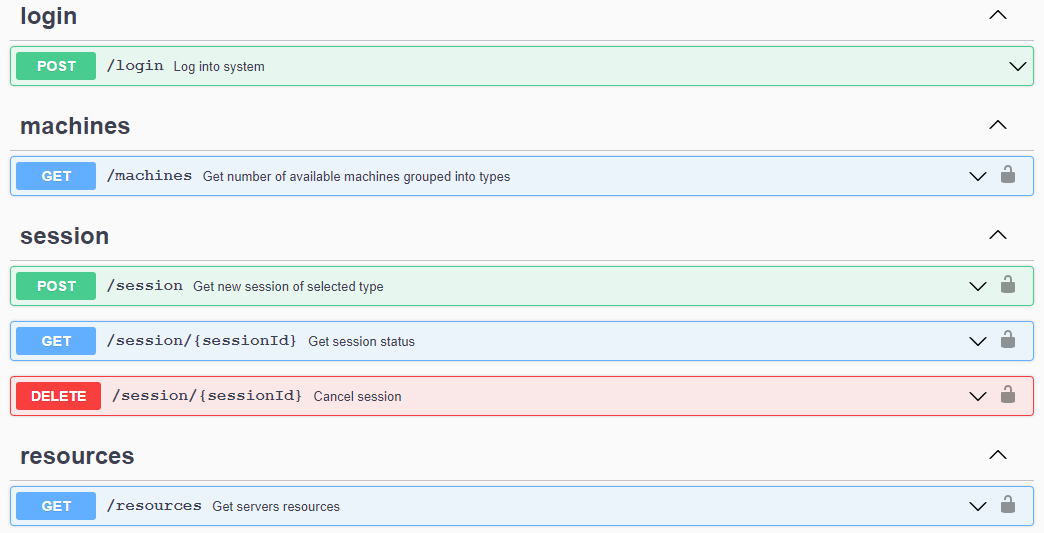
\includegraphics[width=0.9\textwidth]{endpoints.png}
    \caption{Endpointy API}
\end{figure}

\begin{itemize}
    \item Login - służy do logowania do systemu; współdzielony przez aplikację kliencką oraz panel administracyjny. Poprawne zalogowanie zwraca token do dalszej autoryzacji.
    \item Machines - służy do pobierania przez aplikację informacji o typach i ilości dostępnych maszyn. Utworzenie sesji jest możliwe poprzez \texttt{POST} z typem maszyny. W odpowiedzi użytkownik dostaje częściowo wypełniony obiekt sesji zawierający id umożliwiające dalsze zapytania. \texttt{GET} zwraca obiekt sesji z aktualnym stanem. Jeżeli sesja jest gotowa, to zawiera on też adres, z którym należy nawiązać połączenie RDP. Ten endpoint, oraz wszystkie następne wymagają autoryzacji poprzez umieszczenie tokenu otrzymanego podczas logowania w odpowiednim nagłówku wiadomości, oraz dostępne są tylko dla użytkownika.
    \item Session - pozwala na wysłanie prośby o uzyskanie sesji, pobranie stanu sesji oraz jej anulowanie.
    \item Resources - udostępnia informację o zasobach działających serwerów wirtualizacji. Dostępny jedynie dla administratora.
\end{itemize}

\subsection{Komunikacja wewnątrz systemu - broker wiadomości}
\label{communication:broker}

Komunikacja wewnątrz systemu opiera się na kolejkach opisanych w \nameref{external-modules}. W celu uniknięcia wyścigów i utrzymania spójności modelu systemu pomiędzy nadzorcami ustalone są następujące zasady:
\begin{itemize}               
    \item Nadzorca może zmienić stan systemu jedynie w reakcji na odpowiedź serwera wirtualizacji. Odpowiedzi te wysyłane są do wszystkich nadzorców, dzięki czemu każdy nadzorca ma taki sam model systemu.
    \item Wiadomości przetwarzane są przez serwer wirtualizacji w sposób atomowy. Pojedyncza wiadomość musi zostać w pełni obsłużona zanim program przejdzie do obsługi kolejnej.
    \item Serwer wirtualizacji odpowiada na wiadomości wysyłając nowy stan maszyn. Jeżeli żądanie nie może być spełnione z powodu błędnego żądania, to serwer nie odpowiada na żądanie. Wyjątkiem jest żądanie o wysłanie aktualnego stanu maszyn.
    \item Z powodu asynchroniczności wiadomości moduły nie oczekują na odpowiedź. W przypadku nadzorcy przetwarzanie "odpowiedzi" zostanie uruchomione przez zmianę modelu.
    \item Do monitorowania utrzymania połączenia z brokerem użyty jest wbudowany mechanizm, który umożliwia wywołanie odpowiedniej procedury, gdy moduł nie wyśle wiadomości o podtrzymaniu połączenia przez określony czas\footnote{\href{https://www.rabbitmq.com/consumers.html\#active-consumer}{Mechanizm wykrywania aktywności konsumentów w kolejce}}. Używając tego nadzorcy wykrywają, kiedy poszczególne serwery wirtualizacji przestaną działać, a serwery wirtualizacji - kiedy wszyscy nadzorcy przestaną działać.
\end{itemize}

Opisane wyżej założenia pozwalają uniknąć problemu hazardów i wyścigów. Jeżeli wiele nadzorców wyśle do serwera wirtualizacji tą samą prośbę, np. o stworzenie sesji na konkretnej maszynie, to z atomowości obsługi sesja zostanie stworzona tylko dla pierwszego z nich. Serwer wirtualizacji wyśle wiadomość o aktualizacji stanu maszyn i zignoruje pozostałe prośby. Nadzorcy otrzymają zmianę stanów, co spowoduje wywołanie odpowiednich procedur. Dla pierwszego będzie to dalsza część procesu tworzenia sesji, a pozostali nadzorcy pozostaną w procesie wyszukiwania maszyny do sesji.

\subsection{Informacja o działaniu klienta w systemie}

Ważną informacją, która musi posiadać system, to fakt, czy użytkownik rzeczywiście jest podłączony do maszyny wirtualnej.
System uzyskuje ta informację komunikując się z jeszcze jednym brokerem wiadomości, który jest dedykowany do komunikacji z użytkownikami.
Każda aplikacja kliencka po podłączeniu się do maszyny wirtualnej poprzez protokół RDP tworzy kolejkę o takiej nazwie jak uzyskany identyfikator sesji.
Serwer wirtualizacji sprawdza co jakiś czas, czy na końcu kolejki istnieje jakikolwiek konsument.
Gdy użytkownik się rozłączy to kolejka jest usuwana przez aplikację kliencką.

\end{document}